\section{Definitions, Families of Curves}

\subsection{Definitions}

\begin{definition}[Order]
    Order of a DE is the highest-ordered derivative appearing in it.
    So
    \begin{equation}
        \frac{d^2y}{dx^2}+2b(\frac{dy}{dx})^3+y=0
    \end{equation}
    is a 2nd order DE. In general,
    \begin{equation}
        F(x,y,y',y'',\ldots,y^{(n)})=0.
    \end{equation}
    is an $n$-th order DE.
    Under restrictions on $F$, can find a solution in terms of the other $n+1$ variables
    \begin{equation}
        y^{(n)}=f(x,y,y',\ldots,y^{(n-1)}).\label{DESoln}
    \end{equation}
\end{definition}

\begin{definition}[Solution]
    A function $\phi$ on interval $x\in (a,b)$ is a solution to the DE (\ref{DESoln})
    if the $n$ derivatives exist on $x\in(a,b)$ and $\phi^{(n)}(x)=f(x,\phi(x),\ldots,\phi^{(n-1)}(x))$.
\end{definition}

\begin{definition}[First order DE]
    A first order DE is of the form
    \begin{equation}
        \frac{dy}{dx}=f(x,y)
    \end{equation}
    with solution of the form $y=f(x)$.
    Can be rewritten for convenience in the form
    \begin{equation}
        M(x,y)dx+N(x,y)dy=0
    \end{equation}
\end{definition}

\begin{definition}[Linear ODE]
    An ODE of order $n$ is linear if it can be written in the form
    \begin{equation}
        b_0(x)\frac{d^ny}{dx^n}+b_1(x)\frac{d^{n-1}y}{dx^{n-1}}+\cdots+b_{n-1}(x)\frac{dy}{dx}+b_{n}(x)y=R(x)
    \end{equation}
\end{definition}

\begin{definition}[Partial DE]
    Is of the form, for example
    \begin{equation}
        b_0(x,y)\frac{\pr w}{\pr x}+b_x(x,y)\frac{\pr w}{\pr y}=R(x,y)
    \end{equation}
\end{definition}

\subsection{Families of Solutions}

Solutions to the DE
\begin{equation}
    \frac{dy}{dx}=f(x,y)\Leftrightarrow y=\int f(x)dx+c
\end{equation}

exist as one-parameter families with parameter $c$.

\subsection{Isoclines}

Let there be the DE

\begin{equation}
    \frac{dy}{dx}=y
\end{equation}

Isoclines are lines $f(x,y)=y=c$. Example:

\begin{figure}[H]
    \centering
    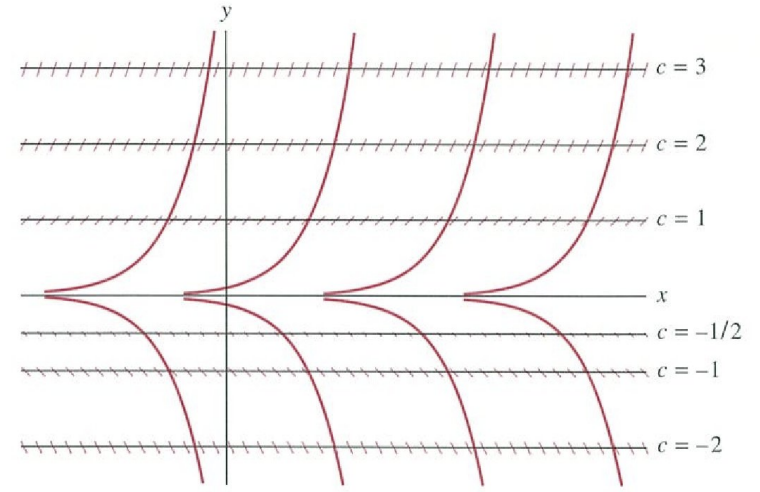
\includegraphics[scale=0.75]{figures/Screen Shot 2021-09-27 at 3.25.57 PM.png}
    \caption{Isoclines of $\frac{dy}{dx}=y$}
\end{figure}

\subsection{Existence Theorem}

Consider equation

\begin{equation}
    \frac{dy}{dx}=f(x,y)
\end{equation}

Further, let $T$ denote the rectangle defined by
\begin{eqnarray}
    |x-x_0|\leq a\\
    |y-y_0|\leq b
\end{eqnarray}
with the point $(x_0,y_0)$ as the center.
Also let $f,\frac{\pr f}{\pr y}$ be continuous functions of $x,y$ in $T$.

With these conditions an interval exists for $x_0$ where $|x-x_0|\leq h$, and function $y(x)$
which has properties
\begin{enumerate}
    \item $y=y(x)$ is a sol'n of the DE on interval $|x-x_0|\leq h$
    \item On this interval, $|y(x)-y_0|\leq b$
    \item $y=y(x_0)=y_0$ at $x=x_0$
    \item $y(x)$ is unique on interval $|x-x_0|\leq h$ where it is the only function with above 3 properties
\end{enumerate}